\subsection{Overview}
\begin{frame}
    \frametitle{Introduction to IDA Pro}
    \begin{itemize}
        \item IDA is \alert{the} tool for reverse engineering
        \item IDA is commercial, costs roughly \$450 US
        \item Scriptable through IDC / IDAPython
        \item Pluggable through a multitude of languages
        \item \alert{Interactive} Disassembler Pro
            \begin{itemize}
                \item It's named interactive for a reason. IDA makes mistakes and won't recognize everything correctly
                \item However, you can interact with the database and correct the errors
            \end{itemize}
        \item FLIRT
            \begin{itemize}
                \item \alert{F}ast \alert{L}ibrary \alert{I}dentification and \alert{R}ecognition \alert{T}echnology
                \item Allows IDA to recognize standard library calls
            \end{itemize}
    \end{itemize}
\end{frame}

\begin{frame}
    \frametitle{Executable Files}
    \mode<article>
    {
        \begin{itemize}
            \item idag.exe: Microsoft Windows GUI
            \item idaw.exe: Microsoft Windows text interface
            \item idau.exe: Microsoft Windows / MSDOS generic text interface
            \item win32\_remote.exe: Remote Windows debugger client
            \item linux\_server / linux\_server64: Remote Linux debugger client
        \end{itemize}
    }
    \mode<presentation>
    {
        idag.exe \dotfill Microsoft Windows GUI                                 \\
        idaw.exe \dotfill Microsoft Windows text interface                      \\
        idau.exe \dotfill Microsoft Windows / MSDOS generic text interface      \\
        win32\_remote.exe \dotfill Remote Windows debugger client               \\
        linux\_server / linux\_server64 \dotfill Remote Linux debugger client
    }
\end{frame}

\begin{frame}
    \frametitle{File Types}
    \mode<article>
    {
        \begin{itemize}
            \item .CFG: Configuration file
            \item .IDC: IDA Script
            \item .IDB: IDA Database
        \end{itemize}
    }
    \mode<presentation>
    {
        .CFG \dotfill Configuration file \\
        .IDC \dotfill IDA Script         \\
        .IDB \dotfill IDA Database       \\
    }
    \begin{itemize}
        \item Processor modules
            \pedbullet{Windows: .W64, .W32, .D32, .DLL}
            \pedbullet{Linux: .IL64, .ILX}
        \item Loader modules
            \pedbullet{Windows: .L64, .LDW, .LDX, .LDO}
            \pedbullet{Linux: .LLX64, .LLX}
        \item Plug-in modules
            \pedbullet{Windows: .P64, .PLW, .PLD, .PL2}
            \pedbullet{Linux: .PLX64, .PLX}
    \end{itemize}
\end{frame}

\begin{frame}
    \frametitle{IDA Autoanalysis Algorithm}
    \begin{block}{}
        The autoanalysis algorithm is not documented, but it can be roughly described as follows (this was verified by Ilfak):
    \end{block}
    \begin{enumerate}
        \item Load the file in the database and create segments
        \item Add the entry point and all DLL exports to the analysis queue
        \item Find all typical code sequences and mark them as code. Add their addresses to the analysis queue
        \item Get an address from the queue and disassemble the code at that address, adding all code references to the queue
        \item While the queue is not empty, go to 4
        \item Make a final analysis pass, converting all unexplored bytes in the text section to code or data
    \end{enumerate}
    \pedref{csw06-sotirov}
\end{frame}

\begin{frame}
    \frametitle{Call Graphs}
    \begin{itemize}
        \item Disassembled binaries can be visualized as graphs
            \pedbullet{Functions represented as nodes}
            \pedbullet{Calls represented as edges}
        \item Useful for viewing the relationships between functions
    \end{itemize}
    \begin{center}
        \uncover{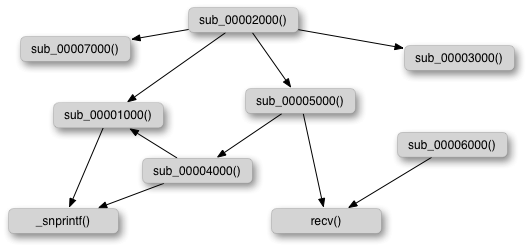
\includegraphics[scale=.40]{images/ida/cfg_call_graph.png}}
    \end{center}
\end{frame}

\begin{frame}[t]
    \frametitle{Control Flow Graphs}
    \begin{columns}
        \column{.6\textwidth}
            \begin{itemize}
                \item Functions can be visualized as graphs
                    \begin{itemize}
                        \item Basic blocks represented as nodes
                        \item Branches represented as edges
                    \end{itemize}
            \end{itemize}
            \begin{center}
                \uncover{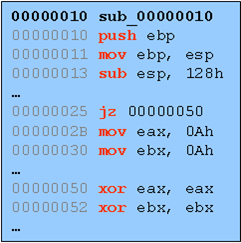
\includegraphics[scale=.30]{images/ida/cfg_deadlisting.png}}
            \end{center}
            \begin{itemize}
                \item Useful for viewing of execution paths
            \end{itemize}
        \column{.4\textwidth}
            \begin{uncoverenv}
                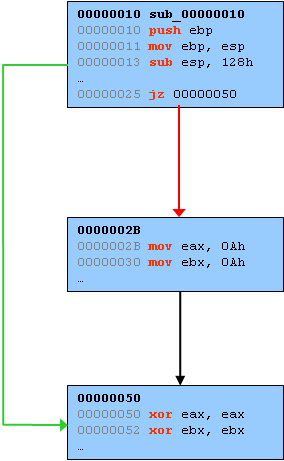
\includegraphics[scale=.40]{images/ida/cfg_graph.png}
            \end{uncoverenv}
    \end{columns}
\end{frame}


\subsection{Overview of Views}
\begin{frame}
    \frametitle{Disassembly View}
    \begin{itemize}
        \item View disassembly, stack offsets, cross refs, strings refs...
        \item Set breakpoints, change names, apply structures edit functions...
    \end{itemize}
    \begin{center}
        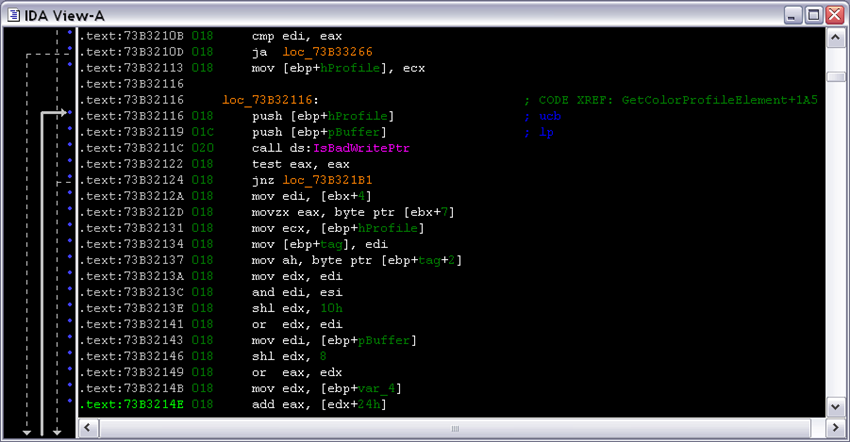
\includegraphics[scale=.75]{images/ida/disasm_view.png}
    \end{center}
\end{frame}

\begin{frame}
    \frametitle{Navigator Band}
    \begin{itemize}
        \item Colorized view of the loaded binary
    \end{itemize}
    \begin{center}
        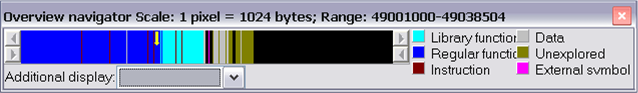
\includegraphics[scale=.50]{images/ida/navigator_band.png} \\
    \end{center}
    \tip{Bands of code that lie interlaced within library functions are probably unrecognized library routines.}
\end{frame}

\begin{frame}
    \frametitle{Messages Window}
    \begin{itemize}
        \item Contains informational messages from IDA
        \item Output from plug-ins
        \item Output from command bar
    \end{itemize}
    \begin{center}
        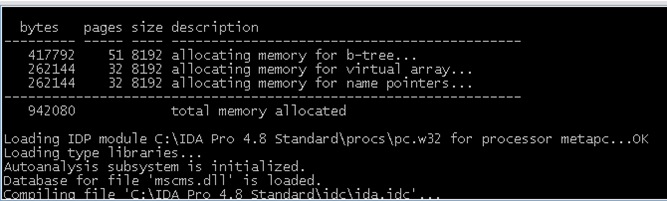
\includegraphics[scale=.50]{images/ida/messages_window.png}
    \end{center}
\end{frame}

\begin{frame}
    \frametitle{Hex View}
    \begin{itemize}
        \item Hex dump of binary
        \item Can be synchronized with disassembly view
    \end{itemize}
    \begin{center}
        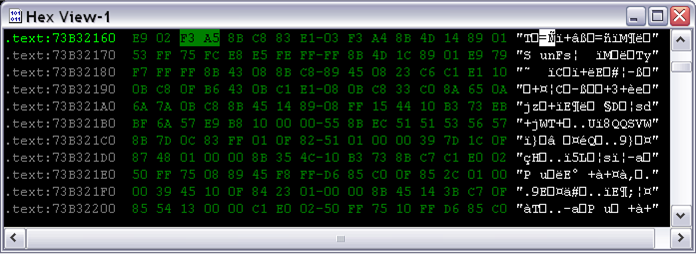
\includegraphics[scale=.60]{images/ida/hex_view.png}
    \end{center}
\end{frame}

\begin{frame}
    \frametitle{Function List}
    List of all functions defined in the current binary
    \begin{center}
        \begin{scriptsize}
        \begin{tabular}{|l|l|}                                                             \hline
            \cellcolor{lightblue}R &  Function returns to caller                           \\ \hline
            \cellcolor{lightblue}F &  Far function                                         \\ \hline
            \cellcolor{lightblue}L &  Library function                                     \\ \hline
            \cellcolor{lightblue}S &  Static Function                                      \\ \hline
            \cellcolor{lightblue}B &  EBP based frame                                      \\ \hline
            \cellcolor{lightblue}T &  Function has type information                        \\ \hline
            \cellcolor{lightblue}= &  Frame pointer is equal to the initial stack pointer  \\ \hline
        \end{tabular}
        \end{scriptsize}
    \end{center}
    \begin{center}
        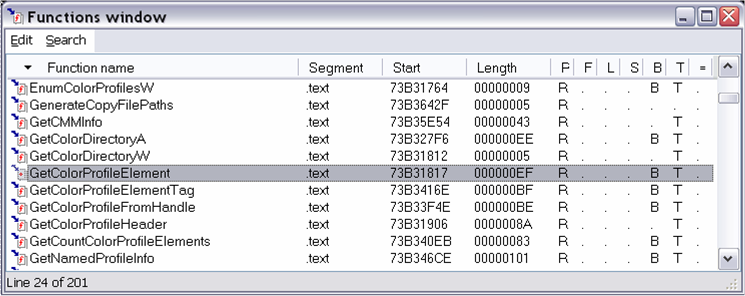
\includegraphics[scale=.50]{images/ida/function_list.png}
    \end{center}
\end{frame}

\begin{frame}
    \frametitle{Names / Symbols List}
    \begin{center}
        \begin{scriptsize}
        \begin{tabular}{|l|l|}                             \hline
            \cellcolor{lightblue}L &  Library function  \\ \hline
            \cellcolor{lightblue}F &  Regular function  \\ \hline
            \cellcolor{lightblue}C &  Instruction       \\ \hline
            \cellcolor{lightblue}A &  ASCII string      \\ \hline
            \cellcolor{lightblue}D &  Data              \\ \hline
            \cellcolor{lightblue}E &  Imported name     \\ \hline
        \end{tabular}
        \end{scriptsize}
    \end{center}
    \begin{center}
        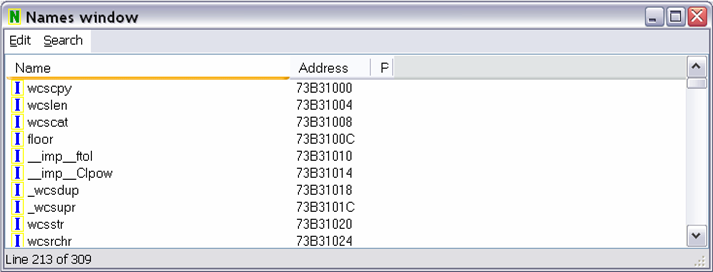
\includegraphics[scale=.50]{images/ida/names_list.png}
    \end{center}
\end{frame}

\begin{frame}
    \frametitle{Imports List}
    \begin{columns}[t]
        \column{.5\textwidth}
            \begin{itemize}
                \item View imported libraries
                \item View imported API
                \item Search
                \item You can make an educated guess of the capabilities and functionality simply by analyzing the import table
            \end{itemize}
        \column{.5\textwidth}
            \begin{center}
                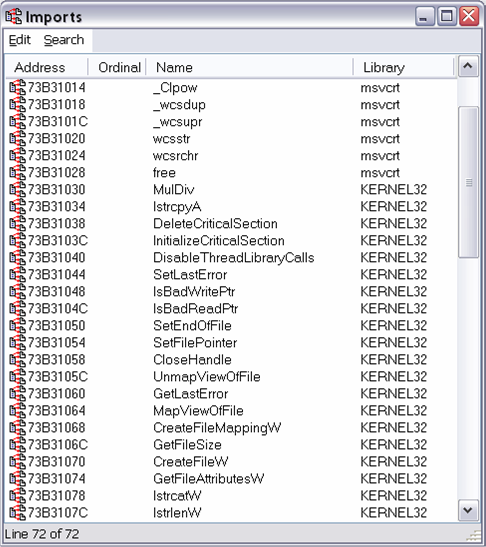
\includegraphics[scale=.50]{images/ida/imports_list.png}
            \end{center}
    \end{columns}
\end{frame}

\begin{frame}
    \frametitle{Strings List}
    \begin{itemize}
        \item View and search the complete list of discovered strings
        \item Take a look at the string list from below. Is it obvious to anyone that some strings are encoded?
    \end{itemize}
    \begin{center}
        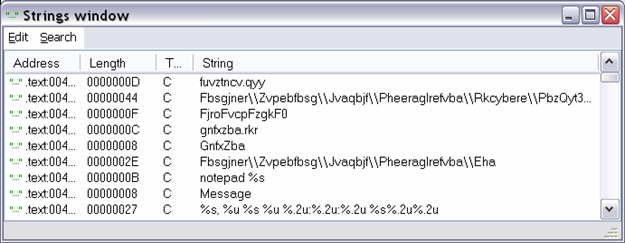
\includegraphics[scale=.85]{images/ida/strings_list.png}
    \end{center}
\end{frame}

\begin{frame}
    \frametitle{Notepad}
    \begin{itemize}
        \item Useful for jotting down notes / comments
        \item Saved in your IDB
    \end{itemize}
    \begin{center}
        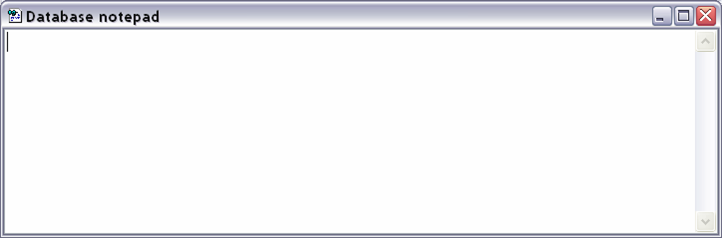
\includegraphics[scale=.50]{images/ida/notepad.png}
    \end{center}
\end{frame}

\begin{frame}
    \frametitle{Debugger}
    \begin{itemize}
        \item Worth mentioning
        \item Personally, I think it's hideous
        \item Key benefits
            \begin{itemize}
                \item Can utilize the power of IDC on breakpoints
                \item Powerful plug-in API
                \item Excellent disassembly base of course
            \end{itemize}
        \item On another note, it is good for ARM (Pocket PC) debugging
            \pedbullet{Pedram's new hobby}
    \end{itemize}
\end{frame}


\subsection{Driving IDA}
\begin{frame}
    \frametitle{Renaming Variables}
    Use the \alert{N} key to rename the argument \\
    \begin{center}
        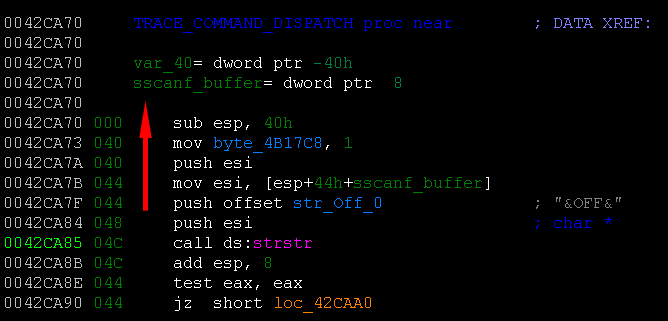
\includegraphics[scale=.50]{images/ida/renaming_variables.png} \\
    \end{center}
\end{frame}

\begin{frame}
    \frametitle{Navigating the Dead Listing}
    \begin{itemize}
        \item CTRL+UP/DOWN to scroll without losing highlight
        \item CTRL+LEFT/RIGHT to jump between items
        \item SHIFT+ENTER to highlight the current item
        \item ALT+UP/DOWN to find the last/next occurrence of the current item
    \end{itemize}
\end{frame}

\begin{frame}
    \frametitle{Marking Positions}
    \begin{itemize}
        \item ALT-M mark position
        \item CTRL-M jump to marked position
        \item To clear marks:
            \pedbullet{Jump $\rightarrow$ Clear mark, then select the mark to erase}
    \end{itemize}
\end{frame}

\begin{frame}
    \frametitle{Cross References}
    \begin{itemize}
        \item Using the Names Window, double click on an API call that you want to find in the target program.  This will highlight the call in the jump table within the disassembly window
        \item Now click on the cross-references button.  This will bring up a cross-references window
        \item By double clicking on the XREF, you will bring focus to the line of code that is making the call
        \item Shortcuts
            \pedbullet{X show all XREFs to operand}
            \pedbullet{CTRL+X show all XREFs to current EA}
    \end{itemize}
\end{frame}

\begin{frame}
    \frametitle{Forward and Backward Navigation}
    \begin{itemize}
        \item By double clicking or highlighting and pressing return, you can follow a XREF directly.
        \item Sometimes multiple XREFs will be shown in the deadlisting
        \item If you have followed multiple XREFs you can navigate back through your XREF history by pressing ESC.
        \item You can navigate forward through your XREF history by pressing CTRL+Enter
        \item Using the arrow keys, the ENTER key, and the ESC key, you can navigate the disassembly view quickly.
    \end{itemize}
\end{frame}


\subsection{Customizations}
\begin{frame}
    \frametitle{Overview}
    \begin{itemize}
        \item Toolbars
        \item Custom desktops
        \item Color palette
            \pedbullet{IDA Pro$\backslash$Customizations$\backslash$IDA Color Palette.reg}
        \item Others (next couple of slides)
            \pedbullet{IDA.CFG}
            \pedbullet{IDAGUI.CFG}
            \pedbullet{IDC scripts and hotkeys (IDA.IDC)}
    \end{itemize}
\end{frame}

\begin{frame}[fragile]
    \frametitle{IDA.CFG}
    \begin{semiverbatim}
        ASCII_PREFIX      = "str."
        MAX_NAMES_LENGTH  = 128
        NameChars         = "$?@>"
        SHOW_XREFS        = 200
        SHOW_BASIC_BLOCKS = YES
        SHOW_SP           = YES
        MangleChars       = "$:?([.)] "
    \end{semiverbatim}
\end{frame}

\begin{frame}[fragile]
    \frametitle{IDAGUI.CFG}
    \begin{semiverbatim}
        HELPFILE              = "c:\\OPS.HLP"
        DISPLAY_PATCH_SUBMENU = YES
        DISPLAY_COMMAND_LINE  = YES
        "ChartXrefsTo"        = "Ctrl-Shift-T"
        "ChartXrefsFrom"      = "Ctrl-Shift-F"
    \end{semiverbatim}
\end{frame}

\begin{frame}[fragile]
    \frametitle{IDA.IDC}
    \begin{semiverbatim}
#include <pedram_function_tagger.idc>
#include <pedram_jump_to_func_top.idc>
#include <pedram_export_disassembly.idc>
#include <pedram_assign_color.idc>

AddHotkey("Ctrl-Shift-X",    "export_disassembly");
AddHotkey("Ctrl-Shift-J",    "jump_to_func_top");
AddHotkey("Ctrl-Shift-Enter","track_follow");
AddHotkey("Ctrl-Shift-N",    "track_name");
AddHotkey("Ctrl-Shift-A",    "hotkey_assign_color");
AddHotkey("Ctrl-Alt-A",      "hotkey_deassign_color");
AddHotkey("Ctrl-Shift-B",    "hotkey_assign_block_color");
AddHotkey("Ctrl-Shift-D",    "hotkey_deassign_block_color");
    \end{semiverbatim}
\end{frame}

\begin{frame}
    \frametitle{Plugins}
    \begin{itemize}
        \item There are a number of plug-ins available
        \item For starters, install pGRAPH.plw
            \pedbullet{Copy it to \%IDA\%$\backslash$plugins}
        \item Use ALT+3 to launch the plug-in
        \item For those of you who are interested, see the next slides for instructions on installing IDA Sync
    \end{itemize}
\end{frame}

\begin{frame}
    \frametitle{Exercise}
    \begin{itemize}
        \item Customize your IDA environment
        \item Install IDA Python and other plug-ins of choice
        \item Use shortcuts!
            \pedbullet{See CD$\backslash$IDA Pro$\backslash$IDA Pro Shortcut Keys Quick Reference.pdf}
    \end{itemize}
\end{frame}
